\documentclass[11pt,a4paper]{article}

\usepackage[utf8]{inputenc}
\usepackage[T1]{fontenc}
\usepackage{lmodern}
\usepackage[english]{babel}
\usepackage[a4paper,top=2.6cm,bottom=2.6cm,left=2.7cm,right=2.7cm]{geometry}
\usepackage{amsmath,amssymb}
\usepackage{graphicx}
\usepackage{booktabs}
\usepackage{multirow}
\usepackage{siunitx}
\usepackage{caption}
\usepackage[table]{xcolor}
\usepackage{enumitem}
\usepackage{microtype}
\usepackage[hidelinks]{hyperref}

\definecolor{univaq}{RGB}{20,60,110}
\captionsetup{font=small,labelfont=bf,width=0.92\linewidth}
\sisetup{detect-weight=true,group-separator={\,}}
\setlist[itemize]{leftmargin=1.4em,itemsep=2pt,topsep=3pt}
\setlist[enumerate]{leftmargin=1.6em,itemsep=3pt,topsep=3pt}

\newcommand{\hvec}{\mathbf{h}}
\newcommand{\xvec}{\mathbf{x}}
\newcommand{\mvec}{\mathbf{m}}
\newcommand{\given}{\mid}

\title{Deep and Probabilistic Completion}
\author{Abid Hossain}
\date{November 2026}

\begin{document}

% ============================== TITLE PAGE ==============================
\begin{titlepage}
\centering
\vspace*{0.6cm}

\rule{0.85\linewidth}{0.6pt}\\[1.6em]

{\Huge\bfseries\color{univaq} Deep and Probabilistic Completion}\\[0.7em]
{\Large Learning an internal representation of partially\\ observed data, and knowing when to distrust it}\\[1.6em]
\rule{0.85\linewidth}{0.6pt}\\[2.2em]

\begin{tabular}{@{}r@{\hspace{1.2em}}l@{}}
\textbf{Dataset} & UCI Bike Sharing (\texttt{hour.csv}) \\
\end{tabular}

\vfill

\begin{tabular}{@{}r@{\hspace{1.2em}}l@{}}
\textbf{Author} & Abid Hossain \\
\end{tabular}

\vspace{1.1em}
\vspace{1.2cm}
\end{titlepage}

\tableofcontents
\newpage

% ============================== 1 ==============================
\section{Problem and formulation}

The task is to build a neural system that (i) learns an internal representation of \emph{partially
observed} data, (ii) produces a probability distribution rather than a point for the quantity it must
complete, and (iii) can be interrogated about whether that distribution deserves trust. The
application is hourly bicycle demand in Washington~D.C.\ (Capital Bikeshare, 2011--2012), where each
hour is a vector of observable covariates together with a demand count that is \emph{never observed}
at prediction time.

\paragraph{Block structure and leakage.}
The observable part of each hour is split into two blocks:
\begin{itemize}
  \item a \emph{temporal} block ($9$ features): cyclic hour, cyclic day-of-week, cyclic day-of-year,
        year, holiday flag, working-day flag;
  \item a \emph{weather} block ($6$ features): temperature, felt temperature, humidity, wind speed,
        and two indicators for the weather situation (\texttt{weathersit}$=2$ and $\ge 3$).
\end{itemize}
The target is the total count \texttt{cnt}. Following the instruction to exclude features that reveal
the target directly, \texttt{casual} and \texttt{registered}
are removed from the input space: they satisfy \texttt{casual} $+$ \texttt{registered} $=$
\texttt{cnt} exactly, so either alone determines the answer. The row index \texttt{instant} and the
date \texttt{dteday} are dropped as identifiers (the date is already encoded by the temporal block).
The exclusion is asserted in code in the accompanying notebook rather than only stated.

\paragraph{Completion as a masked-observation problem.}
Rather than a plain regressor, the model is written as a completion system: the encoder receives the
observed values together with a binary mask,
\begin{equation}
  \hvec = f_\theta\big([\,\xvec \odot \mvec,\; \mvec\,]\big), \qquad \mvec\in\{0,1\}^{15},
\end{equation}
so that missingness is part of the input rather than something the network must infer. One set of
weights therefore defines a \emph{family} of predictors indexed by the observation mask, which is what
makes the experiment of Section~\ref{sec:obs} possible without retraining.

\paragraph{Data quality note.}
The file has \num{17379} rows, i.e.\ \num{165} hours are absent relative to a full two-year calendar,
spread over 76 incomplete days. This matters for the case study in Section~\ref{sec:reliability}: the
storm of 2012-10-29/30 appears in the record mostly \emph{as missing hours}, not as 24 low-count rows.

% ============================== 2 ==============================
\section{Experimental protocol}

\paragraph{Split.}
The split is chronological rather than random: \num{12165} hours for training (2011-01-01 to
2012-05-27), \num{2607} for validation (to 2012-09-12) and \num{2607} for test (2012-09-12 to
2012-12-31). A random split would allow the model to interpolate between adjacent hours of the same
day and would hide the regime change that the uncertainty analysis is about. Standardisation
statistics and the variance temperature of Section~\ref{sec:unc} are fitted on training and
validation data only; the test block is touched once, for evaluation.

\paragraph{Observation generator.}
During training the mask is sampled per example from three regimes: full observation
($p=0.55$), weather block entirely missing ($p=0.30$), and a random partial mask keeping
$50$--$90\%$ of the features ($p=0.15$). At evaluation time the mask is fixed and no sampling
occurs. Model selection uses the validation objective under \emph{full} observation.

\paragraph{Two architectures, one capacity.}
Both encoders have exactly \num{108002} trainable parameters, width 128 and a code of dimension 32, so
the comparison isolates composition:
\begin{itemize}
  \item \textbf{shallow}: $\mathrm{Linear}(30\!\to\!128)\to\mathrm{GELU}\to\mathrm{Linear}(128\!\to\!32)\to\mathrm{GELU}$;
  \item \textbf{deep}: the same input and output layers plus \textbf{three pre-norm residual blocks}
        of width 128 with dropout $0.1$ \cite{he2016}.
\end{itemize}
Both use identical readouts: $\mu(\hvec)$ and $\log\sigma(\hvec)$ from two linear heads.

\paragraph{Training and metrics.}
AdamW, learning rate $5\times10^{-4}$, weight decay $10^{-4}$, batch 256, cosine schedule over at most
300 epochs, early stopping (patience 40) on validation NLL, three seeds per configuration. Point
metrics are reported in bikes per hour after rescaling; the NLL is reported in nats on the
standardised target so that it is comparable across models. Calibration is measured by coverage at
nominal levels, by the probability integral transform (PIT) \cite{dawid1984}, and by the gap between
mean absolute error and reported $\sigma$. All code runs on CPU in about one minute.

% ============================== 3 ==============================
\section{The learned representation}

Because the encoder is trained only to minimise a predictive loss, it is legitimate to ask what it
chose to represent. We probe the frozen code with linear read-outs fitted on training-hour codes and
scored on test-hour codes, and compare against the raw inputs, which are the natural reference: a
feature that is already linearly decodable from $\xvec$ is not a contribution of the encoder.

\begin{table}[t]
\centering
\caption{Linear decodability of attributes from a frozen representation (test accuracy). The raw
inputs are an upper reference, not a competitor: hour, day-of-week, working-day and the bad-weather
flag are literally features of $\xvec$. The informative comparison is between the two codes.}
\label{tab:probes}
\small
\begin{tabular}{lccc}
\toprule
probe task & raw inputs & shallow $\hvec$ & deep $\hvec$ \\
\midrule
hour of day (24 classes)      & 1.000 & 0.872 & 0.747 \\
day of week (7 classes)       & 1.000 & 0.862 & 0.736 \\
working day (2 classes)       & 1.000 & 0.999 & 0.994 \\
bad weather (2 classes)       & 1.000 & 0.999 & 0.995 \\
\midrule
participation ratio of code   & 9.02  & 2.73  & 2.17 \\
\bottomrule
\end{tabular}
\end{table}

Three findings are worth separating. First, the coarse, policy-relevant attributes survive compression
almost losslessly: working-day and bad weather are recovered at $0.99$. Second, the fine-grained
cyclical variable is compressed but not discarded: hour-of-day is recovered at $0.75$ (deep) and
$0.87$ (shallow) against a chance level of $1/24\approx0.04$. Third, and counter-intuitively,
\emph{the deeper code is the less faithful one} while being the better predictor
(Section~\ref{sec:depth}). Depth produced a narrower, more task-specialised summary rather than a
richer one; the participation ratio (the effective number of dimensions used, Table~\ref{tab:probes})
falls from $2.73$ to $2.17$ out of 32.

\begin{figure}[t]
\centering
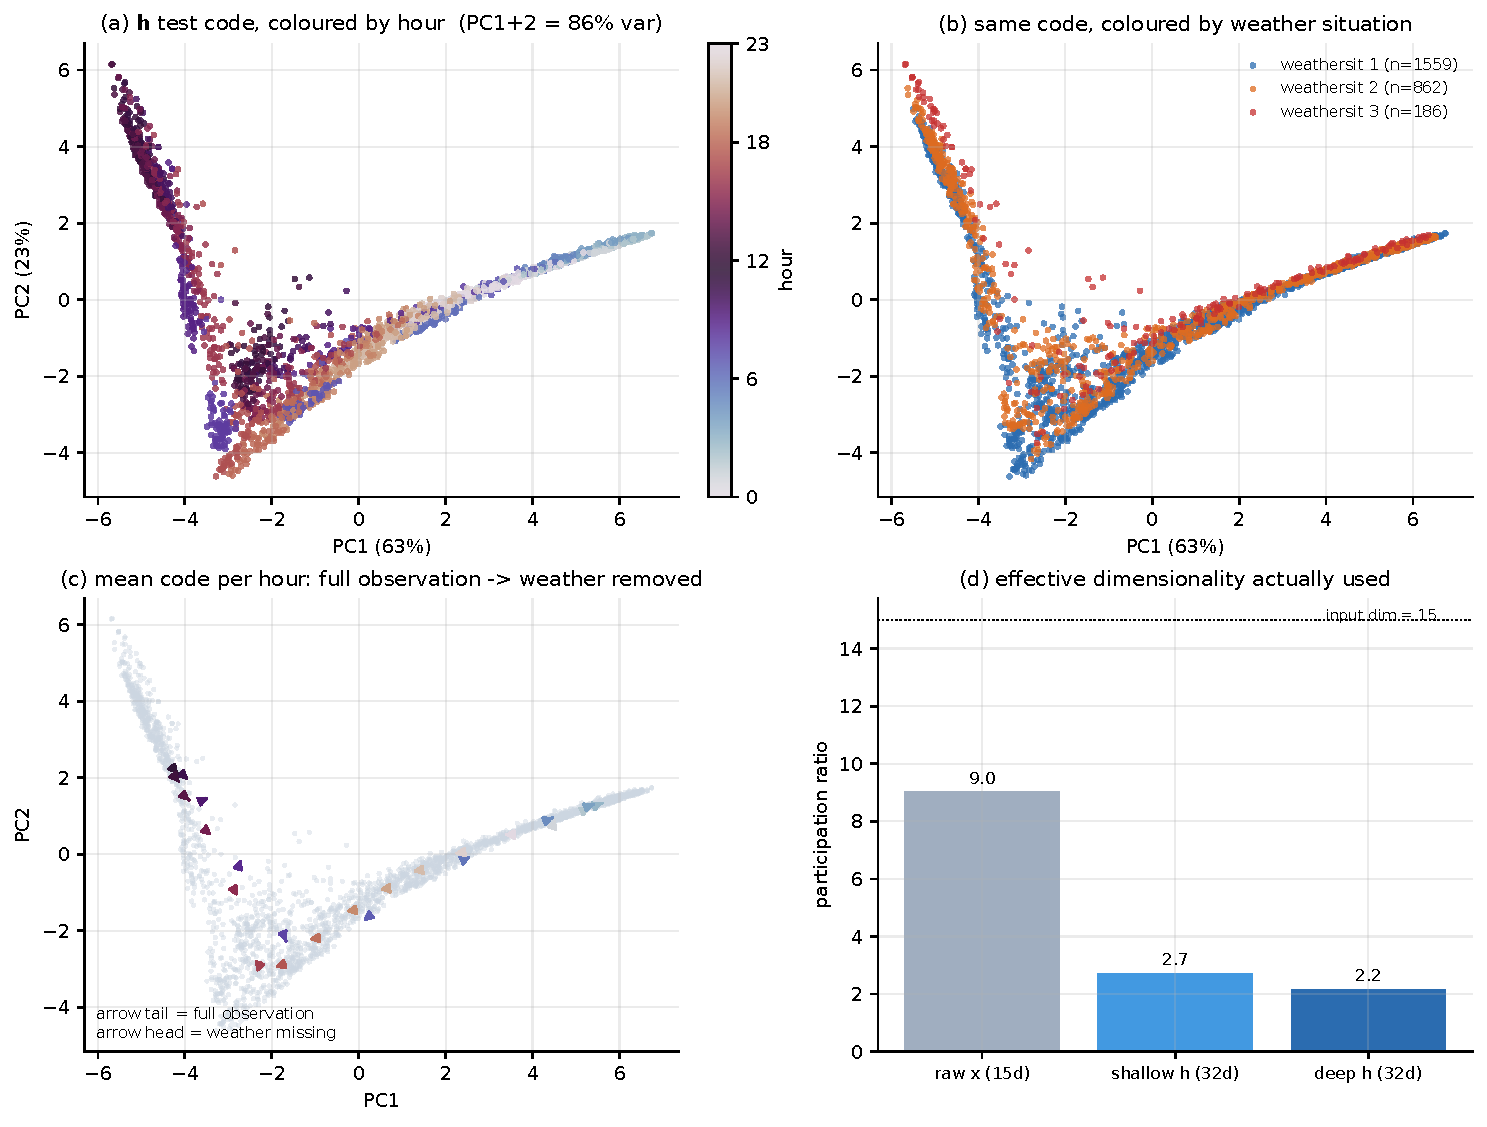
\includegraphics[width=\linewidth]{../figures/fig02_representation.pdf}
\caption{Structure of the code on test hours. (a) PC1 alone orders the hours along two branches of a
fold; PC1+PC2 hold $86.4\%$ of the variance. (b) Weather situation does \emph{not} obtain its own
principal direction --- the colours overlap --- even though it is linearly decodable at $0.99$; the
information lives in the residual directions that PCA discards. (c) Mean code per hour under full
observation (arrow tail) and with the weather block removed (arrow head): the code moves when the
observation changes. (d) Effective dimensionality compared with the $15$-dimensional input.}
\label{fig:repr}
\end{figure}

Figure~\ref{fig:repr} adds two qualitative points and one caution. The code arranges hours on a
\emph{folded one-dimensional manifold} rather than a ring: PCA is a linear projection, and a circular
variable projected linearly appears as a fold. Panel~(b) is the caution --- probes and PCA answer
different questions and here they disagree, so trusting only the scatter plot would miss the weather
information entirely. Panel~(c) is the point that matters for everything that follows: masking the
weather block displaces the mean code of \emph{every} hour. The encoder is a function of the mask, not
only of the hour, which is precisely what a probabilistic readout needs in order to widen when an
input is missing.

% ============================== 4 ==============================
\section{Depth}\label{sec:depth}

\begin{table}[t]
\centering
\caption{Depth comparison on the test block (mean $\pm$ standard deviation over three seeds). Coverage
is the empirical frequency inside the nominal interval; the gap is the mean absolute difference from
nominal over the four levels.}
\label{tab:depth}
\small
\begin{tabular}{lcc}
\toprule
 & shallow & deep \\
\midrule
parameters                   & \num{108002} & \num{108002} \\
RMSE (bikes/h)               & $124.2\pm1.6$ & $104.7\pm4.0$ \\
NLL (nats)                   & $0.971\pm0.028$ & $0.859\pm0.276$ \\
mean $\sigma$ (bikes/h)      & $68.4$ & $51.2$ \\
coverage $50\%$              & $0.427\pm0.013$ & $0.361\pm0.029$ \\
coverage $95\%$              & $0.859\pm0.016$ & $0.818\pm0.050$ \\
mean $|$coverage $-$ nominal$|$ & $0.098$ & $0.149$ \\
hour probe accuracy          & $0.872$ & $0.747$ \\
participation ratio          & $2.73$ & $2.17$ \\
\bottomrule
\end{tabular}
\end{table}

The residual network is the better predictor at identical capacity: RMSE falls by about $16\%$
($124.2\to104.7$) and the NLL by about $12\%$. It can represent the interaction of weather, hour and
day-type that a single non-linearity must approximate with a much smoother function. Two costs are
visible in Table~\ref{tab:depth} and deserve to be reported rather than averaged away. The
seed-to-seed spread of the deep model is about three times larger ($\pm4.0$ vs $\pm1.6$ RMSE): a model
that is better on average is also one whose result depends more on initialisation. And on raw
$\sigma$ the deep model has the \emph{worse} coverage, so depth did not buy calibration. The
temperature analysis of the next section shows that a single scalar repairs the shallow model's
coverage more completely than the deep model's.

\begin{figure}[t]
\centering
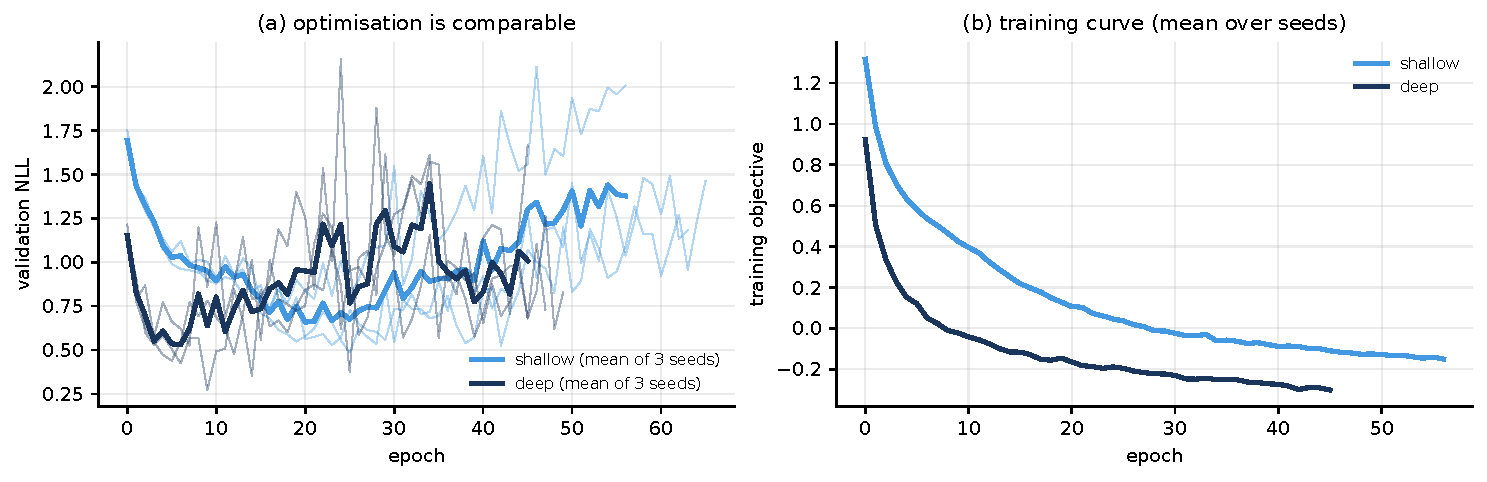
\includegraphics[width=\linewidth]{../figures/fig04_depth_training.pdf}
\caption{Validation NLL and training objective during optimisation, three seeds per architecture.
Early stopping selects a very early checkpoint for both models: the diurnal structure is learned
within a handful of epochs and further training overfits the training hours.}
\label{fig:depthtrain}
\end{figure}

% ============================== 5 ==============================
\section{Probabilistic readout}\label{sec:unc}

\paragraph{Objective.}
The readout predicts the parameters of a Gaussian, $p(y\given\hvec)=\mathcal{N}\big(\mu(\hvec),\sigma^2(\hvec)\big)$,
and is trained by minimising the negative log-likelihood
\begin{equation}
  \mathcal{L}(\theta) \;=\; \frac{(y-\mu(\hvec))^2}{2\sigma^2(\hvec)} \;+\; \log\sigma(\hvec) \;+\; \tfrac12\log 2\pi .
  \label{eq:nll}
\end{equation}
This is not a heuristic loss. Minimising \eqref{eq:nll} over $\sigma$ for fixed $\mu$ gives
$\sigma^2(\hvec)=\mathbb{E}\big[(y-\mu)^2\given\hvec\big]$, i.e.\ the network is trained to predict its
own squared error \cite{nix1994,bishop2006}. The second term is what makes the problem non-trivial: it
charges the model for claiming confidence, so shrinking $\sigma$ is only profitable where the error
really is small. Without it, a mean-squared-error model has exactly \emph{one} global noise level.

\paragraph{Is the readout doing anything?}
The natural ablation is the same deep encoder trained with plain MSE, whose optimal probabilistic
completion is a single constant $\sigma$ fitted on validation residuals. Table~\ref{tab:unc} gives the
answer, and it is more nuanced than expected. The constant-$\sigma$ model is the \emph{most accurate}
($99.8$ vs $104.7$ RMSE) and has the best raw coverage ($0.850$), yet loses decisively on likelihood
($1.119$ vs $0.674$ after temperature). The interpretation is that a single number must be wide enough
for the evening peak and is therefore far too wide at night: it cannot put its width in the right
place, and the likelihood is the only one of these metrics that notices. The probabilistic objective
also costs about $5\%$ of point accuracy, which is a real price and should be stated as such.

\begin{table}[t]
\centering
\caption{Uncertainty ablation on the test block. $\tau$ is a single variance temperature fitted on
validation data by NLL; $\tau=1$ means the network's own $\sigma$ already has the right scale.}
\label{tab:unc}
\small
\begin{tabular}{lcccccc}
\toprule
model & RMSE & NLL & mean $\sigma$ & cov.\,$95\%$ & $\tau$ & NLL\,$\times\tau$ \\
\midrule
shallow, Gaussian NLL          & 124.2 & 0.971 & 68.4 & 0.859 & $1.21\pm0.07$ & 0.754 \\
deep, Gaussian NLL             & 104.7 & 0.859 & 51.2 & 0.818 & $1.15\pm0.17$ & 0.674 \\
deep, MSE ($1$ constant $\sigma$) & 99.8 & 1.119 & 72.9 & 0.850 & --- & --- \\
\bottomrule
\end{tabular}
\end{table}

\paragraph{Temperature.}
Both networks need a modest correction ($\tau\approx1.15$ and $1.21$), i.e.\ both are mildly
over-confident even in distribution, and rescaling recovers most of the missing coverage
($0.818\to0.868$ for the deep model, $0.859\to0.927$ for the shallow one). Separating a wrong
\emph{size} (repairable by a scalar) from a wrong \emph{shape} (not repairable) is the point of this
step, and Section~\ref{sec:reliability} exploits exactly that distinction.

% ============================== 6 ==============================
\section{Varying the observation}\label{sec:obs}

The hidden targets are the same \num{2607} test hours in both conditions; only what the system may see
changes. In condition \textbf{A} (rich) temporal and weather blocks are observed; in condition
\textbf{B} (impoverished) the weather block is masked, as if the weather feed were down while the time
is still known. \emph{No retraining occurs between A and B}: same weights, different mask. This is the
operational meaning of the completion formulation of Section~1. We then go finer than two points and
reveal $k\in\{0,\dots,6\}$ of the six weather features, averaging over all subsets of that size.

\begin{table}[t]
\centering
\caption{Same weights, two observation conditions (mean over three seeds, $\tau$-calibrated).}
\label{tab:obs}
\small
\begin{tabular}{llcccc}
\toprule
architecture & condition & RMSE & mean $\sigma$ & NLL & cov.\,$95\%$ \\
\midrule
\multirow{2}{*}{deep} & A rich (T+W)      & 104.7 & 59.1 & 0.674 & 0.868 \\
                      & B impoverished (T)& 123.1 & 65.6 & 0.875 & 0.835 \\
\midrule
\multirow{2}{*}{shallow} & A rich (T+W)   & 124.2 & 82.5 & 0.754 & 0.927 \\
                         & B impoverished (T) & 139.3 & 95.0 & 0.895 & 0.901 \\
\bottomrule
\end{tabular}
\end{table}

\begin{figure}[t]
\centering
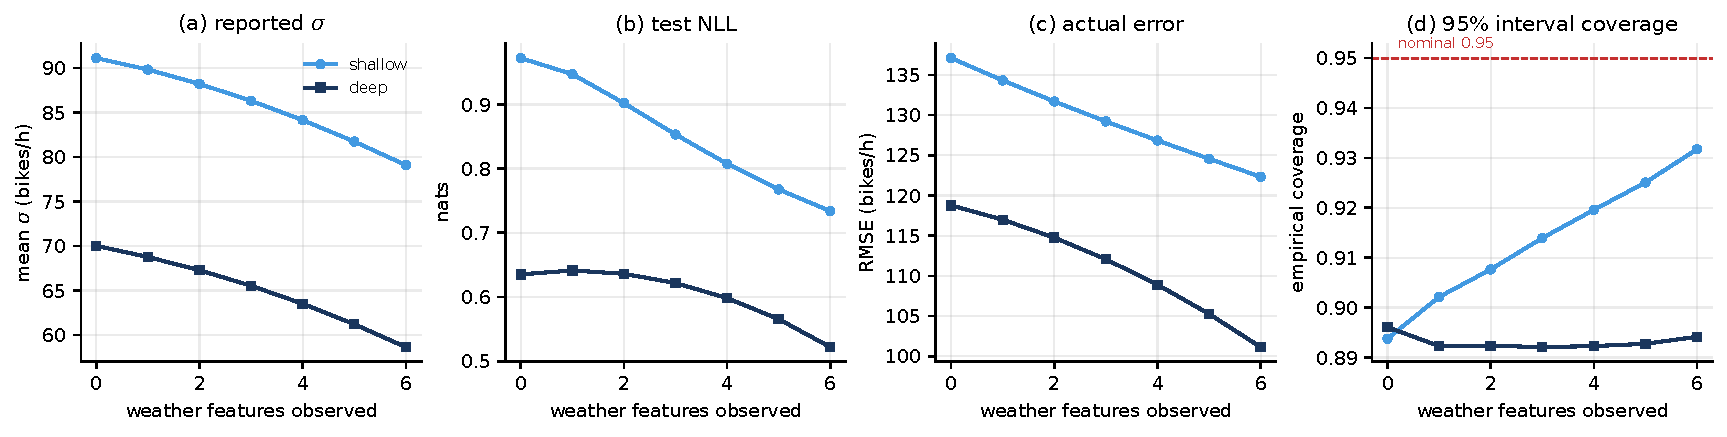
\includegraphics[width=\linewidth]{../figures/fig06_observation.pdf}
\caption{Uncertainty as a function of available information. The temporal block is always observed;
$k$ weather features are revealed, averaged over all subsets of size $k$. Panels (a)--(c) decrease
monotonically; panel (d) compares empirical coverage with the nominal $0.95$.}
\label{fig:obs}
\end{figure}

\begin{table}[t]
\centering
\caption{Graded information sweep for the deep model (seed with best validation NLL), selected points.}
\label{tab:graded}
\small
\begin{tabular}{lccccccc}
\toprule
weather features observed $k$ & 0 & 1 & 2 & 3 & 4 & 5 & 6 \\
\midrule
mean $\sigma$ (bikes/h) & 70.0 & 68.8 & 67.3 & 65.5 & 63.5 & 61.2 & 58.6 \\
RMSE (bikes/h)          & 118.8 & 117.0 & 114.8 & 112.1 & 108.9 & 105.3 & 101.1 \\
\bottomrule
\end{tabular}
\end{table}

Table~\ref{tab:obs} and Figure~\ref{fig:obs} are the central positive result of this work: the
reported uncertainty tracks the information that was actually removed, monotonically, and nothing in
the objective told the model which sensors were more informative. Removing the whole weather block
raises $\sigma$ by $11\%$ and the NLL by $0.20$ for the deep model, and the graded sweep in
Table~\ref{tab:graded} is monotone in $k$ for both $\sigma$ and the error. The shallow model behaves
the same way from a higher level ($91.1\to79.1$).

Two caveats are necessary, and both are visible in panel~(d). First, panels (a) and (c) respond to the
same mask, so their agreement shows that the model is \emph{responsive}, not that its numbers are
\emph{right}; the within-condition test is Section~\ref{sec:reliability}, and that is the test which
can fail. Second, $\sigma$ remains too small in absolute terms everywhere: at $k=0$ the model reports
$70$ while making an error of $119$, and coverage never reaches the nominal $0.95$ --- for the deep
model it is essentially flat at $\approx0.89$ across the whole sweep. Making a model more uncertain
does not make it calibrated.

% ============================== 7 ==============================
\section{Reliability: one informative case, two misleading ones}\label{sec:reliability}

All diagnostics below use the $\tau$-calibrated predictive distribution of the deep model on the test
block.

\subsection{Global picture}

\begin{figure}[t]
\centering
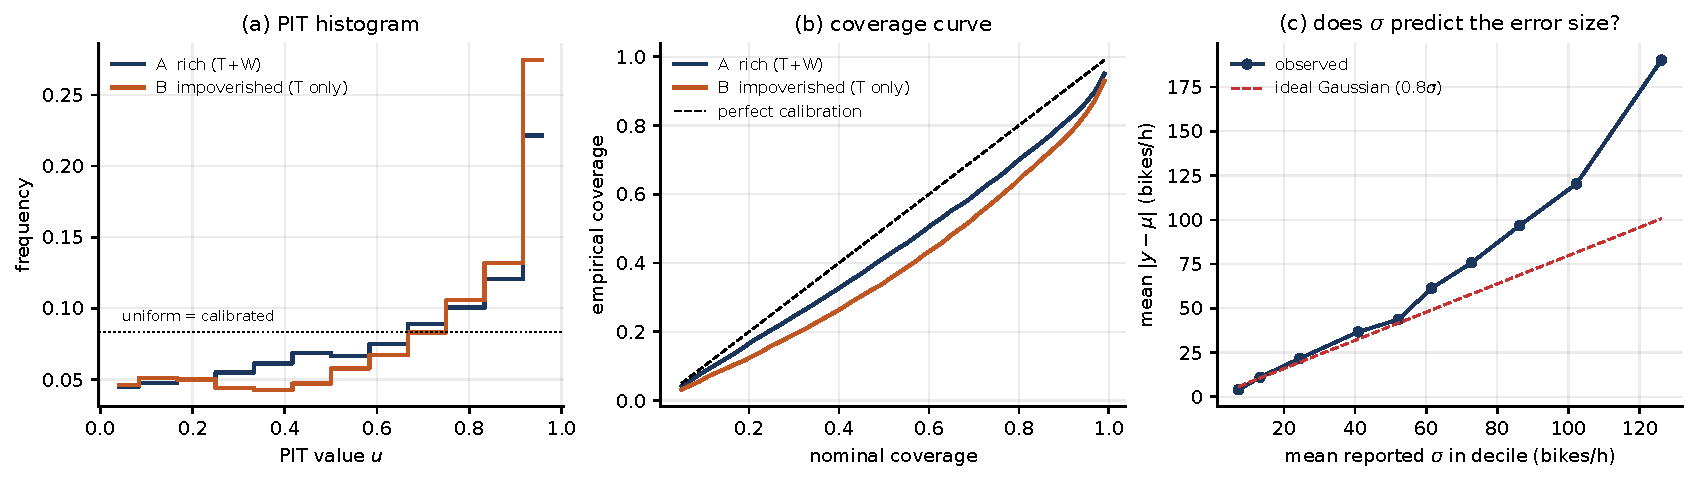
\includegraphics[width=\linewidth]{../figures/fig07_reliability.pdf}
\caption{(a) PIT histogram: uniform would mean calibration. (b) Coverage curve against nominal level.
(c) Reported $\sigma$ in deciles against the mean absolute error in that decile, with the ideal
Gaussian relation $\mathbb{E}[|y-\mu|]=0.8\sigma$.}
\label{fig:rel}
\end{figure}

The PIT histogram is strongly $\cup$-shaped: about $5\%$ of hours fall in the lowest bin but $22\%$ in
the highest, against $8.3\%$ for uniformity. The coverage curve lies below the diagonal everywhere ---
a nominal $50\%$ interval covers about $36\%$. The asymmetry is as informative as the miscalibration:
far more mass at $u\approx1$ than at $u\approx0$ means the model far more often \emph{under}-predicts a
large count than over-predicts a small one, which is the signature of fitting a symmetric Gaussian to
a right-skewed, non-negative count. No amount of $\sigma$ fitting repairs a specification error of
that kind \cite{gneiting2007}.

One result went against my expectation and is reported as such: removing the weather block makes the
histogram \emph{worse} ($27\%$ in the top bin, lower coverage). The model does widen its intervals, but
the errors widen faster. Responsiveness is not calibration.

\subsection{The informative case: $\sigma$ ranks difficulty correctly}

Panel~(c) asks the scale-free question: do hours that receive a large $\sigma$ actually go wrong? The
curve is monotone, and two summaries confirm it is not accidental: the Spearman correlation between
$\sigma$ and $|\epsilon|$ is $0.73$ under rich observation and $0.76$ under impoverished observation,
and the fraction of the largest $10\%$ errors that fall inside the largest $10\%$ of $\sigma$ is
$0.52$ ($0.48$ in the impoverished condition) against $0.10$ for random selection. The model does know
\emph{where} it will be wrong --- that is what makes such a system usable for triage, and it is a
genuine property of the learned noise field rather than of the marginal error distribution.

Its failure is in the \emph{magnitude}: the observed curve in panel~(c) lies above the ideal
$0.8\sigma$ line and diverges, reaching about $1.5\sigma$ in the top decile. $\sigma$ is right about
the order of difficulty and wrong about the amount.

\subsection{First misleading case: it is least trustworthy where it matters most}

\begin{table}[t]
\centering
\caption{Reliability by part of the day (deep model, rich observation, $\tau=1.06$ for this seed).
``Viol.'' is the percentage of hours outside the $95\%$ band, nominally $5\%$.}
\label{tab:groups}
\small
\begin{tabular}{lccccccc}
\toprule
group & $n$ & RMSE & MAE & MAPE\,\% & mean $\sigma$ & cov.\,$95\%$ & viol.\,\% \\
\midrule
night (00--05)        & 645 & 19.2  & 10.6  & 70.5 & 13.7  & 0.978 & 2.0 \\
morning peak (06--09) & 432 & 126.9 & 86.0  & 46.0 & 70.1  & 0.854 & 13.9 \\
midday (10--15)       & 651 & 105.2 & 83.3  & 32.2 & 74.0  & 0.853 & 14.7 \\
evening peak (16--19) & 439 & 159.3 & 128.1 & 40.8 & 100.2 & 0.806 & 18.5 \\
late (20--23)         & 440 & 50.4  & 40.5  & 38.0 & 49.0  & 0.959 & 4.1 \\
\midrule
overall               & \num{2607} & 101.1 & 66.1 & --- & 58.6 & 0.894 & 10.3 \\
\bottomrule
\end{tabular}
\end{table}

Figure~\ref{fig:hourly}(a) looks reassuring --- $\sigma$ follows the diurnal cycle --- but the
\emph{gap} between the two curves is the finding. Around 03:00--04:00 the model reports
$\sigma\approx15$ and errs by $\approx20$: nearly right. At 08:00 and 17:00 it reports
$\sigma\approx95$ and $\approx112$ against a per-hour RMSE of $\approx215$: roughly half the width it
should have. Table~\ref{tab:groups} puts this on a probability scale: $2.0\%$ of night hours fall
outside the $95\%$ band (slightly conservative), but $13.9\%$ at the morning peak and $18.5\%$ at the
evening peak, i.e.\ $2.8$ and $3.7$ times the nominal rate, on the largest errors of the day.

The failure is therefore not uniform over-confidence: it is concentrated in the rush hours, which are
exactly the hours for which a demand forecast would be commissioned. An operator who reads
$\sigma=100$ at 17:00 and plans for $\pm200$ is relying on an interval that covers $80.6\%$ of
outcomes rather than $95\%$. The mechanism is the specification error identified above: peak demand is
right-skewed and bounded at zero, and a symmetric likelihood cannot put more than half its mass above
the mean, so it systematically under-predicts the large days.

Note that this is \emph{not} an absolute-versus-relative illusion. At night the MAPE is high ($70\%$)
but $\sigma$ is proportionally large too ($0.45\times$ mean demand), so those intervals do cover. The
peaks are a genuine coverage failure, not a change of units --- a distinction that a single headline
reliability number would have hidden.

\begin{figure}[t]
\centering
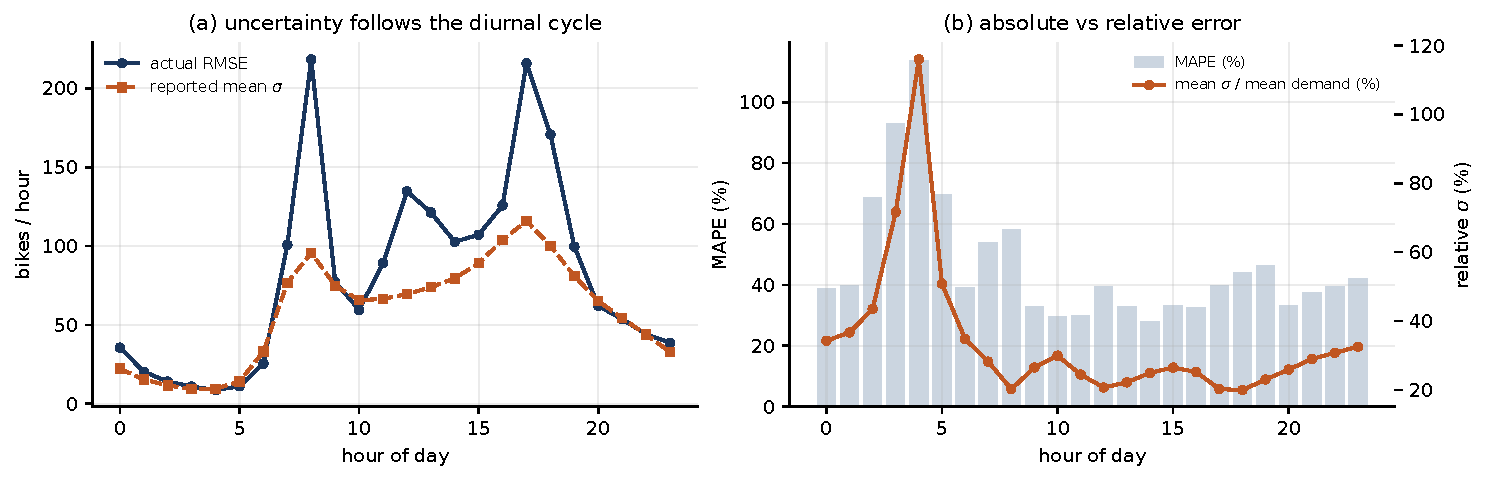
\includegraphics[width=\linewidth]{../figures/fig08_hourly.pdf}
\caption{(a) Per-hour RMSE against per-hour mean reported $\sigma$. (b) Mean absolute percentage error
(bars, left axis) against $\sigma$ relative to mean demand (line, right axis).}
\label{fig:hourly}
\end{figure}

\subsection{Second misleading case: a regime the covariates cannot describe}

Hurricane Sandy reached Washington D.C.\ on 2012-10-29 and the data set's own documentation flags the
day as an anomaly. What the record contains is not 24 hours of low demand but an \emph{outage}: 1 of 24
hours on 10-29 and 11 of 24 on 10-30 are present at all --- the station went offline at 01:00 on the
29th and returned at 13:00 on the 30th. The surviving hours carry collapsed counts (22 rentals at
00:00 on the 29th; an evening peak of 143 where a normal October weekday peaks near 525), while their
covariates look like an ordinary wet Monday --- \texttt{weathersit} never exceeds 3 and wind reaches
$0.36$ of its range. The honest question is therefore not whether the model can predict the storm (36
of the 48 hours do not exist to be predicted) but whether $\sigma$ warns about the 12 hours that do.

\begin{figure}[t]
\centering
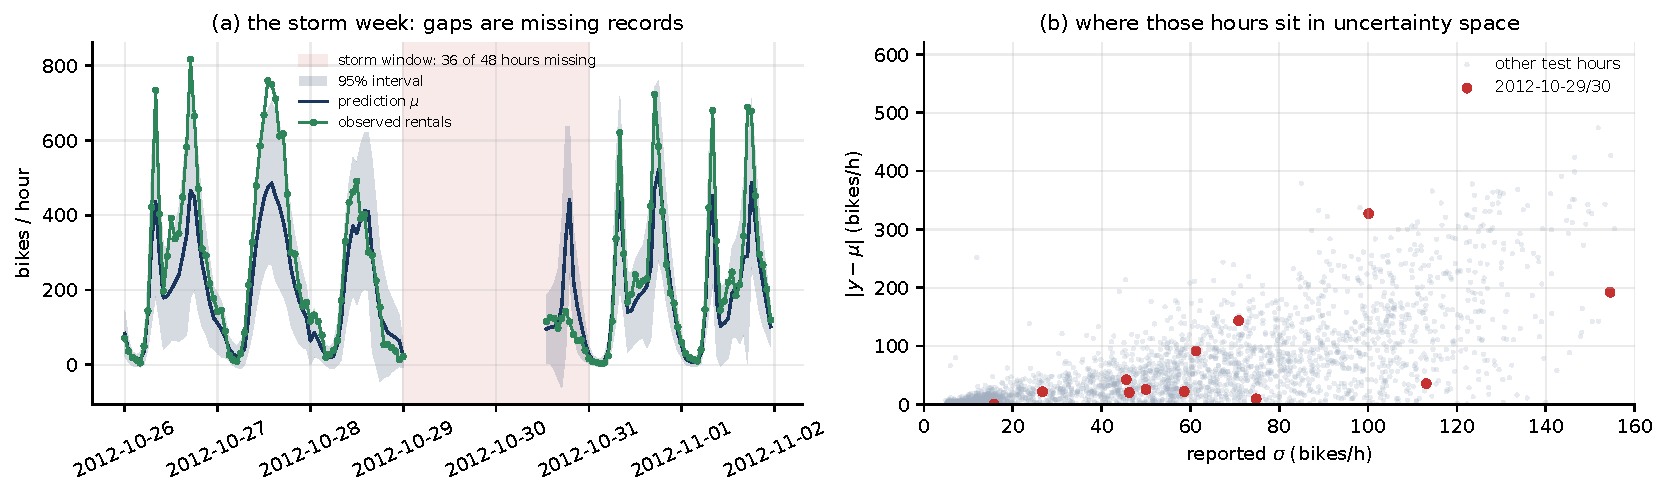
\includegraphics[width=\linewidth]{../figures/fig09_storm.pdf}
\caption{(a) The storm week. Gaps are missing records, not low demand: 36 of the 48 hours in the
shaded window are absent. (b) The surviving storm hours in uncertainty space.}
\label{fig:storm}
\end{figure}

The answer is: partially. Across those 12 hours $\sigma$ did widen --- $68.1$ against $58.6$ for the
test window as a whole --- because \texttt{weathersit}$=3$ with high humidity and wind is a pattern the
training data contains. On average the model over-predicts by $70\%$ ($159.5$ against $93.2$
observed), and its mean absolute error of $77.8$ is only $1.14\sigma$, so most hours stay inside the
band. But 2 of the 12 hours ($17\%$) fall outside the $95\%$ interval and the worst is missed by
$3.3\sigma$ (predicted $442$, observed $115$, $\sigma=100$).

The verdict is \emph{partially informative but systematically biased}: $\sigma$ reacted to the weather
signature it had seen before and could not react to the two things that mattered --- an outage and a
$70\%$ collapse in demand --- because neither leaves a trace in the input vector. The interval stayed
statistically respectable while the point forecast was wrong by a factor of $1.7$.

\paragraph{The statistical version of the same failure.}
The second case does not have to rest on one anecdote. The \emph{same} model is nearly calibrated on
validation hours and degrades on the future block:

\begin{center}
\small
\begin{tabular}{lcc}
\toprule
 & validation (in-distribution) & test (future block) \\
\midrule
coverage $95\%$                & 0.966 & 0.894 \\
P$(\,|err|>2\sigma\,)$         & $3.2\%$ & $10.3\%$ \\
mean $\sigma$ (bikes/h)        & 70.4 & 58.6 \\
RMSE (bikes/h)                 & 87.3 & 101.1 \\
\bottomrule
\end{tabular}
\end{center}

Seven points of coverage are lost and the violation rate more than triples, without the architecture
changing at all. Coverage is a property of the model \emph{and} of the data it is asked about; a
reliability diagram computed on a random split would have reported none of this.

\subsection{What the two failures have in common}

They fail for different reasons, which is the useful part:

\begin{center}
\small
\begin{tabular}{p{3.1cm}p{5.2cm}p{5.2cm}}
\toprule
 & \textbf{rush hours} & \textbf{Sandy window} \\
\midrule
reported $\sigma$ & large ($\approx95$--$112$) & widened by $16\%$ ($58.6\to68.1$) \\
actual error & RMSE $\approx215$ per hour, largest of the day & level bias of $+70\%$ \\
what $\sigma$ gets wrong & the \emph{shape}: symmetric head, skewed target & the \emph{regime}: inputs look normal \\
assumption that breaks & Gaussian likelihood & exchangeability with the training set \\
what would repair it & count or log-normal head; quantile/CRPS objective & epistemic uncertainty, OOD detection, a covariate marking the event \\
\bottomrule
\end{tabular}
\end{center}

What they share is that \emph{neither is repaired by a better-calibrated scalar $\sigma$}. The
temperature $\tau$ was fitted on validation data and can know about neither: it is one number, while
both defects are conditional on the hour and on the regime. This is the practical form of the
aleatoric/epistemic distinction \cite{kendall2017}: $\sigma(\hvec)$ estimates
$\mathbb{E}[(y-\mu)^2\given\hvec]$ \emph{under the training distribution}, and Sandy is not noise but
distribution shift. A conditional-variance head has no access to it, and neither does any calibration
technique that assumes exchangeability \cite{guo2017}.

% ============================== 8 ==============================
\section{Conclusions}

\begin{enumerate}
\item \textbf{A representation is learned and can be inspected.} The 32-dimensional code keeps the
coarse policy-relevant attributes almost losslessly ($0.99$) and compresses the fine-grained cyclical
one ($0.75$ deep, $0.87$ shallow, chance $0.04$). It organises time on a folded one-dimensional
manifold, and it moves when the observation changes --- the encoder is a function of the mask, not only
of the hour.

\item \textbf{Depth buys predictive quality, not calibration.} At identical parameter counts the
residual network lowers RMSE by $\approx16\%$ and NLL by $\approx12\%$, but it has the worse raw
coverage and three times the seed variance. ``Deeper is better calibrated'' is a hypothesis this
experiment rejects.

\item \textbf{The probabilistic readout earns its place, at a price.} A constant $\sigma$ is more
accurate and marginally better covered, yet loses badly on likelihood. The learned $\sigma$ field buys
a usable likelihood and a usable ranking of hard hours for about $5\%$ of point accuracy.

\item \textbf{Reducing observation raises uncertainty monotonically and in the right order.} With fixed
weights, masking the weather block raises $\sigma$ by $11$--$15\%$ and NLL by $0.14$--$0.20$; revealing
weather features one at a time walks $\sigma$ down from $70.0$ to $58.6$ while the error falls from
$118.8$ to $101.1$.

\item \textbf{Uncertainty is informative about ranking and misleading about scale.} $\sigma$ orders the
errors well (Spearman $0.73$--$0.76$; top-decile capture $0.52$ against $0.10$), but it is
systematically too narrow: $22\%$ of PIT mass sits in the top bin, the mean absolute error reaches
$\approx1.5\sigma$ in the highest-$\sigma$ decile, the rush hours violate their $95\%$ band
$14$--$19\%$ of the time while quiet nights are almost perfectly covered, and during the Sandy outage
the model was biased by $+70\%$ while its interval still looked respectable.

\item \textbf{Summary.} This system knows how noisy the world it was trained on is, and can report that
per input --- including, to a useful degree, when an input is missing. It does not know when the world
has changed. Separating those two is the difference between a probabilistic model and a trustworthy
one, and it is why the diagnostics of Section~\ref{sec:reliability}, not the RMSE of
Section~\ref{sec:depth}, should decide whether such a model ships.
\end{enumerate}

% ============================== 9 ==============================
\section{Reproducibility}

\paragraph{Deliverables.}
\texttt{probabilistic\_completion.ipynb} is self-contained and executes top to bottom
(downloading \texttt{hour.csv} if absent), regenerating every figure in \texttt{figures/} and
recording every headline number in \texttt{results/results.json}; every value quoted in this report is
produced by that notebook.

\paragraph{Software.}
Python 3.11; PyTorch for the models and training; NumPy and pandas for data handling; scikit-learn for
the linear probes, PCA and the gradient-boosting reference model used to sanity-check the achievable
error level (test RMSE $\approx95$ bikes/h, which places the deep network's $104.7$ near but not at the
practical ceiling); SciPy for normal quantiles and rank correlations; Matplotlib for figures.
Total runtime is about one minute on CPU.

\paragraph{Seeds and selection.}
Three seeds per architecture, mean $\pm$ standard deviation reported where meaningful. Early stopping
and all model selection use validation NLL under full observation. The reference model for the per-hour
and per-group analysis is the deep network with the best validation NLL.

\begin{thebibliography}{9}
\bibitem{fanaee2013} H.~Fanaee-T and J.~Gama. Event labeling combining ensemble detectors and
background knowledge. \emph{Progress in Artificial Intelligence}, 2(2):113--127, 2013.
\bibitem{bishop2006} C.~M. Bishop. \emph{Pattern Recognition and Machine Learning}. Springer, 2006.
\bibitem{nix1994} D.~A. Nix and A.~S. Weigend. Estimating the mean and variance of the target
probability distribution. In \emph{Proc.\ ICNN}, 1994.
\bibitem{kendall2017} A.~Kendall and Y.~Gal. What uncertainties do we need in Bayesian deep learning
for computer vision? In \emph{NeurIPS}, 2017.
\bibitem{guo2017} C.~Guo, G.~Pleiss, Y.~Sun and K.~Q. Weinberger. On calibration of modern neural
networks. In \emph{ICML}, 2017.
\bibitem{gneiting2007} T.~Gneiting and A.~E. Raftery. Strictly proper scoring rules, prediction, and
estimation. \emph{JASA}, 102(477):359--378, 2007.
\bibitem{dawid1984} A.~P. Dawid. Present position and potential developments: some personal views.
Statistical theory: the prequential approach. \emph{JRSS A}, 147(2):278--292, 1984.
\bibitem{he2016} K.~He, X.~Zhang, S.~Ren and J.~Sun. Deep residual learning for image recognition.
In \emph{CVPR}, 2016.
\bibitem{lakshminarayanan2017} B.~Lakshminarayanan, A.~Pritzel and C.~Blundell. Simple and scalable
predictive uncertainty estimation using deep ensembles. In \emph{NeurIPS}, 2017.
\end{thebibliography}

\end{document}
